\documentclass{beamer}
\usepackage[latin1]{inputenc}

\usetheme{Madrid}
\usecolortheme{default}
\usepackage{amsmath}
\usepackage{amssymb,amsfonts,amsthm}
\usepackage{txfonts}
\usepackage{tkz-euclide}
\usepackage{listings}
\usepackage{adjustbox}
\usepackage{array}
\usepackage{tabularx}
\usepackage{gvv}
\usepackage{lmodern}
\usepackage{circuitikz}
\usepackage{tikz}
\usepackage{graphicx}
\usepackage{gensymb}
\usepackage{physics}

\setbeamertemplate{page number in head/foot}[totalframenumber]

\usepackage{tcolorbox}
\tcbuselibrary{minted,breakable,xparse,skins}



\definecolor{bg}{gray}{0.95}
\DeclareTCBListing{mintedbox}{O{}m!O{}}{%
  breakable=true,
  listing engine=minted,
  listing only,
  minted language=#2,
  minted style=default,
  minted options={%
    linenos,
    gobble=0,
    breaklines=true,
    breakafter=,,
    fontsize=\small,
    numbersep=8pt,
    #1},
  boxsep=0pt,
  left skip=0pt,
  right skip=0pt,
  left=25pt,
  right=0pt,
  top=3pt,
  bottom=3pt,
  arc=5pt,
  leftrule=0pt,
  rightrule=0pt,
  bottomrule=2pt,
  toprule=2pt,
  colback=bg,
  colframe=orange!70,
  enhanced,
  overlay={%
    \begin{tcbclipinterior}
    \fill[orange!20!white] (frame.south west) rectangle ([xshift=20pt]frame.north west);
    \end{tcbclipinterior}},
  #3,
}
\lstset{
    language=C,
    basicstyle=\ttfamily\small,
    keywordstyle=\color{blue},
    stringstyle=\color{orange},
    commentstyle=\color{green!60!black},
    numbers=left,
    numberstyle=\tiny\color{gray},
    breaklines=true,
    showstringspaces=false,
}
\title{2.10.54}
\date{18th september, 2025}
\author{Tammineedi Rushil Shanmukha Srinivas - EE25BTECH11057}

\begin{document}

\frame{\titlepage}
\begin{frame}{Question}
let $\vec{a, b,c}$ be unit vectors such that $\vec{a}+\vec{b}+\vec{c}=\vec{0}$. Which of the following are correct?\\
\begin{enumerate}
    \item $\vec{a}\times \vec{b}=\vec{b}\times \vec{c}=\vec{c}\times \vec{a}=\vec{0}$
    \item $\vec{a}\times \vec{b}=\vec{b}\times \vec{c}=\vec{c}\times \vec{a}\neq \vec{0}$
    \item $\vec{a}\times \vec{b}=\vec{b}\times \vec{c}=\vec{a}\times \vec{c}\neq \vec{0}$
    \item $\vec{a}\times \vec{b},\vec{b}\times \vec{c}, \vec{c}\times \vec{a}$ are mutually perpendicular.
\end{enumerate}
\end{frame}

\begin{frame}{Cross Product and Gram Matrix}

Given ,
\begin{align}
\vec{a}+\vec{b}+\vec{c} = \vec{0} , \norm{\vec{a}} = \norm{\vec{b}} = \norm{\vec{c}} = 1
\end{align}
\begin{align}
(\vec{a}+\vec{b}+\vec{c})^2 = 0
\end{align}
\begin{align}
{\norm{\vec{a}}}^2+{\norm{\vec{b}}}^2+{\norm{\vec{c}}}^2+2\vec{a}^\top\vec{b}+2\vec{b}^\top\vec{c}+2\vec{c}^\top\vec{a} = 0
\end{align}
\begin{align}
\vec{a}^\top\vec{b}+\vec{b}^\top\vec{c}+\vec{c}^\top\vec{a} = \frac{-3}{2}
\end{align}
\begin{align}
\vec{a}+\vec{b}+\vec{c}=\vec{0} \Longrightarrow \myvec{\vec{a} & \vec{b} & \vec{c}}\myvec{1 \\1\\1} = \vec{0} \Longrightarrow
\vec{A}\vec{x} = \vec{0} 
\end{align}
\begin{align}
\vec{A}^\top\vec{A}\vec{x} = \vec{0} \Longrightarrow G\vec{x}=\vec{0}
\end{align}
\end{frame}
\begin{frame}
\begin{align}
\myvec{
\norm{\vec{a}}^2 & \vec{a}^\top\vec{b} & \vec{c}^\top\vec{a} \\
\vec{a}^\top\vec{b} & \norm{\vec{b}}^2 & \vec{b}^\top\vec{c} \\
\vec{c}^\top\vec{a} & \vec{b}^\top\vec{c} & \norm{\vec{c}}^2 }
\myvec{
1 \\ 1 \\ 1} = \vec{0}
\end{align}
\begin{align}
\myvec{
1+\vec{a}^\top\vec{b}+\vec{c}^\top\vec{a} \\
\vec{a}^\top\vec{b}+1+\vec{b}^\top\vec{c} \\
\vec{c}^\top\vec{a}+\vec{b}^\top\vec{c}+1} = \myvec{0 \\ 0 \\ 0}
\end{align}
\begin{align}
1+\vec{a}^\top\vec{b}+\vec{c}^\top\vec{a} = \vec{a}^\top\vec{b}+1+\vec{b}^\top\vec{c} = 
\vec{c}^\top\vec{a}+\vec{b}^\top\vec{c}+1
\end{align}
\begin{align}
\vec{a}^\top\vec{b} = \vec{b}^\top\vec{c} = \vec{c}^\top\vec{a} 
\end{align}
From (4.4)
\begin{align}
\vec{a}^\top\vec{b} = \vec{b}^\top\vec{c} = \vec{c}^\top\vec{a} = \frac{-1}{2}
\end{align}
\begin{align}
\vec{a}^\top\vec{b} = \vec{b}^\top\vec{c} = \vec{c}^\top\vec{a} \Longrightarrow \vec{a}\times\vec{b} = \vec{b}\times\vec{c} = \vec{c}\times\vec{a}
\end{align}
\begin{align}
\vec{a}\times\vec{b} = \vec{b}\times\vec{c} = \vec{c}\times\vec{a} \neq \vec{0}
\end{align}


\end{frame}


\begin{frame}[fragile]
    \frametitle{C Code}
    \begin{lstlisting}
#include <stdio.h>

// Function to compute cross product of two vectors
void cross(double u[3], double v[3], double result[3]) {
    result[0] = u[1]*v[2] - u[2]*v[1];
    result[1] = u[2]*v[0] - u[0]*v[2];
    result[2] = u[0]*v[1] - u[1]*v[0];
}

int main() {
    // Example unit vectors at 120° apart in the xy-plane
    double a[3] = {1.0, 0.0, 0.0};
    double b[3] = {-0.5, 0.86602540378, 0.0};   // cos120, sin120
    double c[3] = {-0.5, -0.86602540378, 0.0};  // cos240, sin240

    double ab[3], bc[3], ca[3];
\end{lstlisting}
\end{frame}
\begin{frame}[fragile]
\begin{lstlisting}
    cross(a, b, ab);
    cross(b, c, bc);
    cross(c, a, ca);

    printf("a × b = (%lf, %lf, %lf)\n", ab[0], ab[1], ab[2]);
    printf("b × c = (%lf, %lf, %lf)\n", bc[0], bc[1], bc[2]);
    printf("c × a = (%lf, %lf, %lf)\n", ca[0], ca[1], ca[2]);

    return 0;
}

    \end{lstlisting}
\end{frame}

\begin{frame}[fragile]
    \frametitle{Python Code 1}
    \begin{lstlisting}
    import ctypes
import math

# Load shared library
lib = ctypes.CDLL("./libcross.so")

# Define function signature
lib.compute_crosses.argtypes = [
    ctypes.POINTER(ctypes.c_double),   # a
    ctypes.POINTER(ctypes.c_double),   # b
    ctypes.POINTER(ctypes.c_double),   # c
    ctypes.POINTER((ctypes.c_double*3)*3)  # result[3][3]
]

# Define the vectors (unit vectors, 120° apart in xy-plane)
a = (ctypes.c_double * 3)(1.0, 0.0, 0.0)
b = (ctypes.c_double * 3)(-0.5, math.sqrt(3)/2, 0.0)
c = (ctypes.c_double * 3)(-0.5, -math.sqrt(3)/2, 0.0)
\end{lstlisting}
\end{frame}
\begin{frame}[fragile]
\begin{lstlisting}
# Prepare result storage (3x3 array of doubles)
ResultArray = (ctypes.c_double * 3) * 3
result = ResultArray()

# Call the C function
lib.compute_crosses(a, b, c, result)

# Print results
print("a × b =", [result[0][i] for i in range(3)])
print("b × c =", [result[1][i] for i in range(3)])
print("c × a =", [result[2][i] for i in range(3)])

    \end{lstlisting}
\end{frame}

\begin{frame}[fragile]
    \frametitle{Python Code 2}
    \begin{lstlisting}

import matplotlib.pyplot as plt
import numpy as np
from mpl_toolkits.mplot3d import Axes3D

# Define the vectors (unit vectors 120° apart in xy-plane)
a = np.array([1.0, 0.0, 0.0])
b = np.array([-0.5, np.sqrt(3)/2, 0.0])
c = np.array([-0.5, -np.sqrt(3)/2, 0.0])

# Cross product (all same)
ab = np.cross(a, b)

# Create 3D plot
fig = plt.figure(figsize=(7,7))
ax = fig.add_subplot(111, projection="3d")
# Plot vector a (red arrow)
ax.quiver(0,0,0, *a, color="r")
\end{lstlisting}
\end{frame}
\begin{frame}[fragile]
\begin{lstlisting}
ax.text(a[0], a[1], a[2], "a", color="r")
# Plot vector b (green thick line)
ax.plot([0, b[0]], [0, b[1]], [0, b[2]], color="g", linewidth=3)
ax.text(b[0] + 0.2, b[1], b[2], "b", color="g")   # label moved right
# Plot vector c (blue arrow)
ax.quiver(0,0,0, *c, color="b")
ax.text(c[0] - 0.2, c[1], c[2], "c", color="b")   # label moved left
# Plot cross product vector (black arrow)
ax.quiver(0,0,0, *ab, color="k", linestyle="dashed")
ax.text(ab[0], ab[1], ab[2], "a×b = b×c = c×a", color="k")

# Axes settings
ax.set_xlabel("X")
ax.set_ylabel("Y")
ax.set_zlabel("Z")
ax.set_xlim([-1.5, 1.5])
ax.set_ylim([-1.5, 1.5])
ax.set_zlim([0, 1.2])
ax.set_title("Vectors a, b, c and Cross Products")
plt.savefig("../figs/figb.png")
plt.show()

    \end{lstlisting}
\end{frame}

\subsection{Plots}
\begin{frame}
\frametitle{Plots}
\begin{figure}
\centering
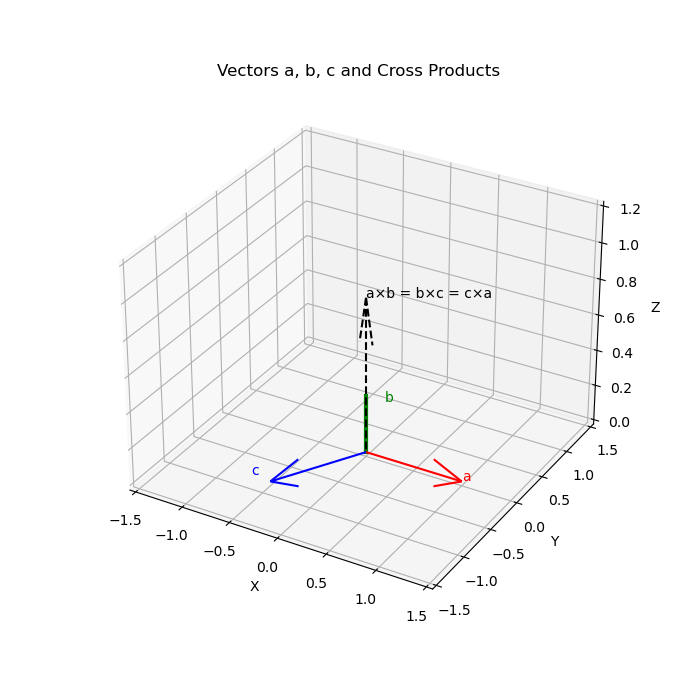
\includegraphics[width=0.55\columnwidth]{figs/figb.png}
\caption{fig : Representation of vectors}
\label{Fig8}
\end{figure}
\end{frame}




\end{document}